\chapter{EVALUATION} 
\label{sec.evaluation}
In this section, we demonstrate SOAR's utility by implementing three example use cases that together ``play'' different types of its API: comparing the performance of 2.4 GHz and 5 GHz bands, studying channel survey statistics and home wireless environment. Our goal is to illustrate how \sysname can support a variety of measurement needs.
\section{Method}
\subsection{Measurements}
\label{ssec.measurements}

We perform both active and passive measurements of network traffic from home wireless access point and correlate those measurements with the wireless metrics for the corresponding traffic. Passive measurements reflect the actual performance more accurately. Unlike passive measurement, active measurements generate additional network traffic that are sent over the network to, for example, measuring the time it takes for the packet to reach the other end of the network (TCP RTT) and the available capacity of a wireless network. However, active measurements might introduce contention or disturb the normal traffic flow. Combining active and passive measurements is called hybrid measurements. 

To generate the maximum possible send/receive rate that \sysname can achieve. we use \texttt{socket.send}/\texttt{socket.recv} within a tight loop and using a timer to saturate the available network bandwidth. We perform all tests between clients on the same wireless network and the home access point. We collect network traffic statistics and channel survey information from both wireless interfaces on the access point. The data collection on the access point is done by periodically querying some data exposed by our platform's supported API (e.g, \texttt{get\_network\_bytes} and \texttt{wifi\_status}). Our sandbox environment ensure that monitoring should not have any negative impact on the routers. 
 
\subsection{Deployment Experience}
\label{ssec.deployment}

We deploy our platform on a TP-Link TL-WDR3600 router, which has a 560 MHz MIPS processor, 8MB of flash storage, 128MB of RAM and a dual-band wireless interface. We replace the router's default software with a custom version of OpenWrt Chaos Calmer~\cite{openwrt}. The 802.11 interface operates at both 2.4 GHz and 5 GHz bands. The location is in NYU campus, which is an office building. 

\subsection{Metrics}
\label{ssec.metrics}

Our metrics are based on supported APIs provided by \sysname. We use channel busy time as an indicator of the channel utilization, and with channel transmit time and receive time to calculate the external interference. We also report the achieved throughput generated by the running experiments. We next elaborate on our metrics.

\textbf{Channel busy time:} The channel busy time is the amount of time the primary channel was sensed busy. This seems to be about the same as the sum of channel transmit and receive times, unless there is a lot of external interference (like another busy Wi-Fi network on the same channel)\cite{channelsurvey}. We report the channel busy time every 30 seconds. Typically, a lower channel busy time is an indicator of good throughput and negligible interference.

\textbf{Channel transmit and receive time:} The channel transmit and receive time are the amount of time the radio spent transmitting and receiving data. In general, the following relation seems to be like that: 

\(\frac{t_{channel-tx} + t_{channel-rx}}{t_{channel}} < \frac{t_{channel-busy}}{t_{channel}} < 100\%\).

\textbf{Achieved throughput:} Our platform periodically (30 seconds) reports the actual throughput for each interfaces. Achieved throughput is the actual total number of bytes over time, and it captures the actual demand on the wireless network. This metric depends on the experiment's data rate and is bounded by the wireless effective throughput. The throughput is computed as the transmitted bytes over one second period.

\textbf{TCP round-trip time (RTT):} RTT is the difference between the time of the data and TCP SYN packets and its corresponding acknowledgements. As this RTT increases, it can have an adverse impact on performance, especially for applications that are latency sensitive. Measuring the RTT between the access point and the home devices is important for us to understand wireless performance.

\textbf{Additional metrics:} Our platform reports each station's \texttt{tx} retries and \texttt{tx} failed. \texttt{tx} retries and \texttt{tx} failed are reported only in downlink (gateway to station) and we use them as an additional performance indicator. Finally, our platform also reports unix timestamp along with other metrics. This is used to help me calculate throughput and study network usage pattern. 

\section{Usecase: Comparing the wireless performance of 2.4 GHz and 5 GHz bands}
\label{sec.usecase1}

Better use of 5 GHz to improve wireless performance on a dense WiFi network is a common strategy because there are generally fewer devices in the 5 GHz band (This means that the noise floor is much lower) and 5 GHz band has less non-WiFi interference. Thus our hypothesis was that devices on the 5 GHz band would perform better.

We use \sysname to evaluate the wireless performance of network traffic on 2.4 GHz and 5 GHz band. Our focus is not on improving performance, but rather to underscore how we can use \sysname to gain useful insights into a real network.

For this experiment, the router that we use enables both 2.4 GHz and 5 GHz radios, which allows us to compare the performance of these two bands. To ensure there are similar network traffic on 2.4 GHz and 5 GHz band, we performed a multi-threaded TCP experiment on \sysname to send intermittent TCP packets to clients which connected 2.4 GHz and 5 GHz band, respectively. Then we collect network traffic statistics to compare wireless network performance.

\begin{figure}
\begin{subfigure}{0.5\textwidth}
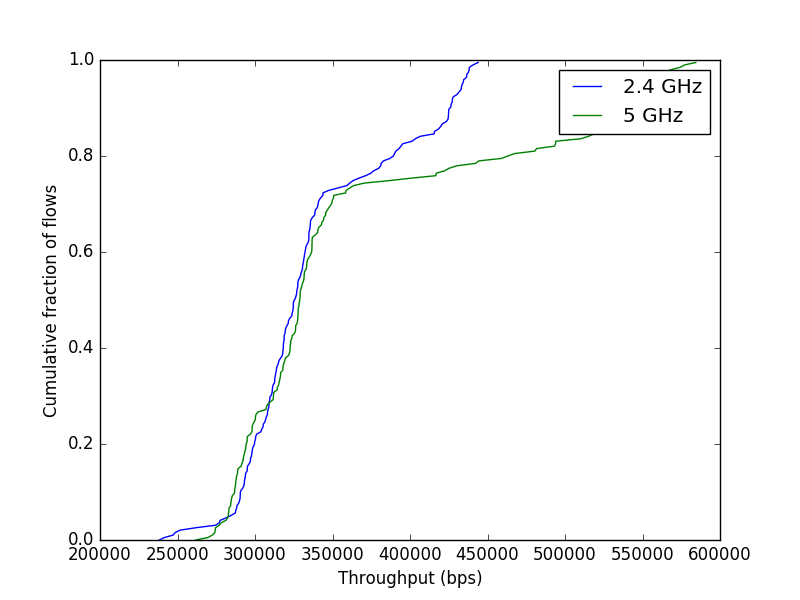
\includegraphics[width=\linewidth]{figure/throughput(5g_vs_2g).png}
\caption{Network traffic in the 5 GHz band achieve higher throughput} 
\label{fig:throughput}
\end{subfigure}
\hspace*{\fill} % separation between the subfigures
\begin{subfigure}{0.5\textwidth}
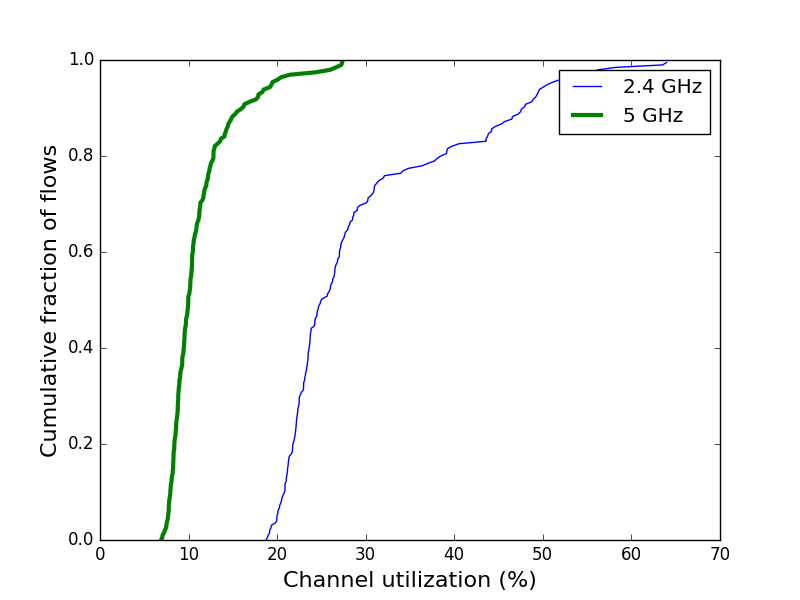
\includegraphics[width=\linewidth]{figure/channel_utilization(2g_vs_5g).png}
\caption{Network traffic in the 2.4 GHz band experience higher channel utilization.} 
\label{fig:utilization}
\end{subfigure}
\hspace*{\fill} % separation between the subfigures
\begin{subfigure}{0.45\textwidth}
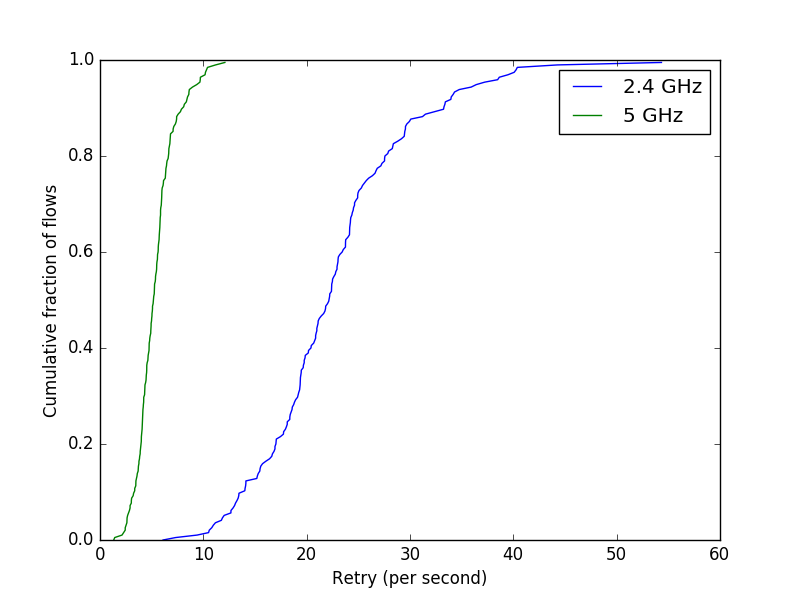
\includegraphics[width=\linewidth]{figure/retries(2g_vs_5g).png}
\caption{Network traffic in the 2.4 GHz band experience higher tx retries.} 
\label{fig:retries}
\end{subfigure}
\hspace*{\fill} % separation between the subfigures
\begin{subfigure}{0.5\textwidth}
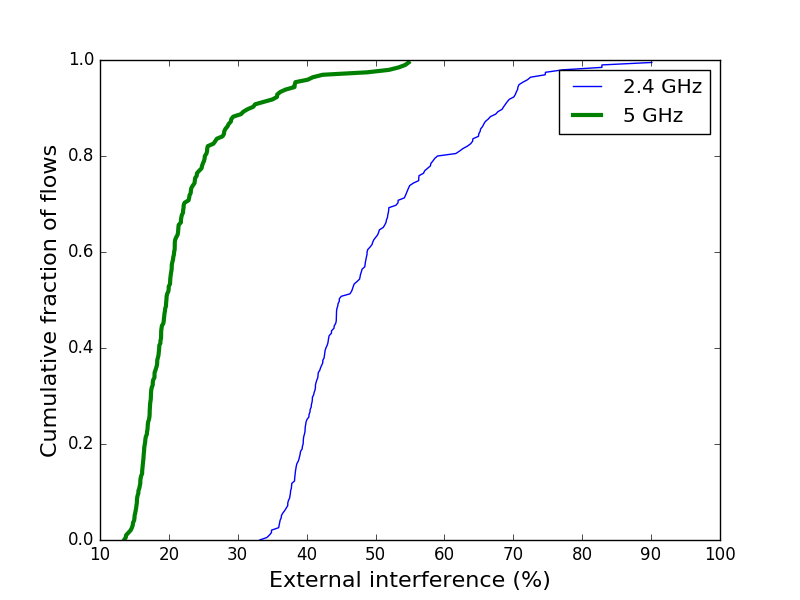
\includegraphics[width=\linewidth]{figure/external_interference(2g_vs_5g).png}
\caption{Network traffic in the 5 GHz band has less external interference.} 
\label{fig:interference}
\end{subfigure}
\caption{Characteristics of flows in the 5 GHz vs. the 2.4 GHz spectrum.} 
\label{fig:5gvs2g}
\end{figure}

\textbf{2.4 GHz vs. 5 GHz:} We use throughput, channel utilization, retransmission times and external interference as our indicator of wireless performance because we can obtain these metrics easily from our supported APIs. We calculate throughput as follows: using \texttt{get\_network\_bytes} to provide TCP statistics. We study the aggregate TCP throughput achieved during the captured lifetime of the network traffic. We compute the average throughput at every one-second interval by the divisor of aggregate TCP throughput and the difference between the correspond timestamp. \texttt{get\_station} can help us obtain the number of retry packets at each clients. We also compute channel utilization and external interference as the percentage of channel busy time and external interference time in any given one-second interval. 

We see that the use of 5 GHz improves performance, reducing channel utilization, external interference and retransmission rate. Figure \ref{fig:throughput} shows the network traffic in the 5 GHz band achieve higher throughput. Figure \ref{fig:utilization} shows the channel utilization in 2.4 GHz are much higher than 5 GHz. Figure \ref{fig:retries} shows the retransmission times per 40 seconds; the result shows that transmissions are more common in the 2.4 GHz band. Figure \ref{fig:interference} plots the CDF of the external interference for all network traffic for both the 2.4 GHz band and the 5 GHz bands. The 5 GHz band has less interference as signal does not propagate well through walls. A limiting factor to identify the real wireless performance is the lack of contention and feedback from external sources (i.e., local contention and non-WiFi wireless devices). However, we still leverage channel busy time to detect airtime utilization.

\begin{figure}
\centering
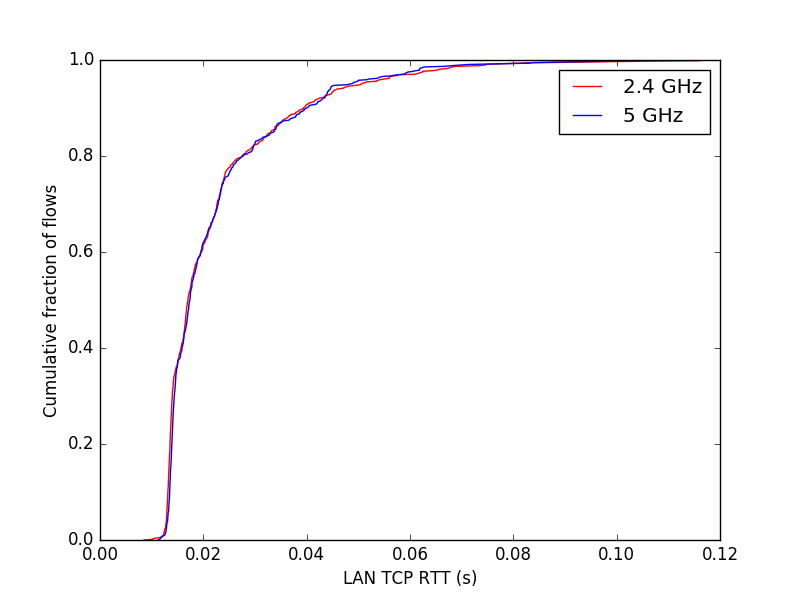
\includegraphics[width=0.5\textwidth]{figure/tcp_rtt.png}
\caption{LAN TCP round-trip time for different bands (e.g,. 2 GHz, 5 GHz).} 
\label{fig:tcprtt}
\end{figure}

\textbf{TCP round-trip time is similar on 2.4 GHz and 5 GHz band.} We calculate TCP round-trip time as follows: using the home router as vantage point and calculate the time between a TCP packet coming and its respective TCP acknowledgement from a connected client. We collected the TCP round-trip between the wireless home router and a wireless client on 2.4 GHz and 5 GHz band. Figure \ref{fig:tcprtt} plots the CDF of the TCP round-trip times for all network traffic for both the 2.4 GHz band and the 5 GHz band. The result shows that TCP round-trip time on 2.4 GHz and 5 GHz band are similar.

\begin{figure}
\centering
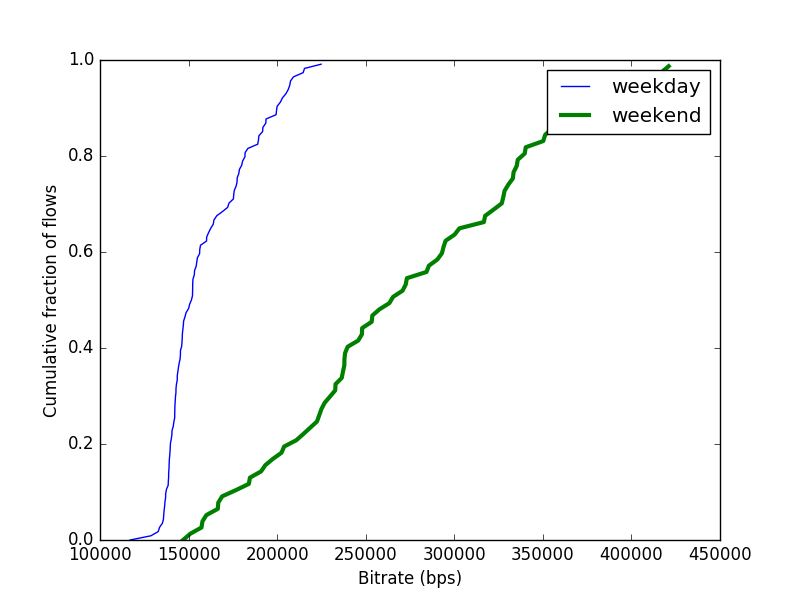
\includegraphics[width=0.5\textwidth]{figure/bitrate(weekday_vs_weekend).png}
\caption{Bitrate on weekday and weekend in an office building in NYU Brooklyn campus. Weekend bitrate is more than weekday bitrate.} 
\label{fig:compare}
\end{figure}  

\section{Usecase: Studying channel survey statistics}
\label{sec.usecase2}

\begin{figure}
\centering
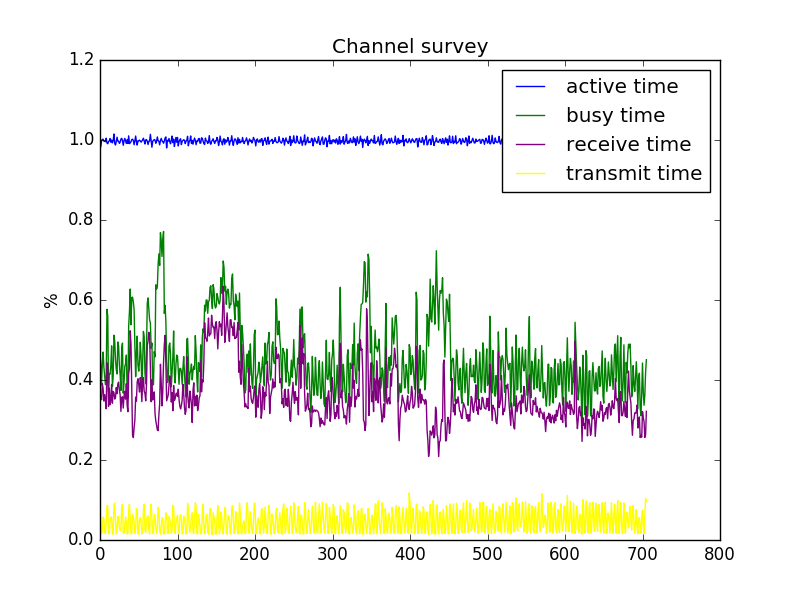
\includegraphics[width=0.5\textwidth]{figure/channel.png}
\caption{Channel survey metrics in 2.4 GHz band through \texttt{wifi\_status}.} 
\label{fig:channelsurvey}
\end{figure}

Measurement studies show that congestion in a wireless network leads to lower overall network throughput and capability. The lack of techniques to identify and characterize congestion in wireless networks has prevented relevant research. To better understand congestion in wireless networks, \sysname provides the capabilities to explore radio channel channel utilization data. 

As \cite{channelsurvey} did before, we replicated this experiment through our \sysname platform. We use \texttt{wifi\_status} to collect channel busy time, active time, transmit time and receive time. Figure \ref{fig:channelsurvey} shows the channel survey statistics captured in 2.4 GHz band. We find that channel active time is the same as running time if you don't change channels. Channel busy time seems to be the same as the sum of transmit time and receive time, unless there is a lot of external interference (e.g, heavy external traffic on the same channel, non-WiFi devices).

Next, we study the potential indicator can cause the degradation of a wireless performance. We therefore investigate this, by correlating the throughput (which can be caused by interference) with the airtime utilization and external interference. Interestingly, we find that there is no strong correlation between wireless performance and airtime utilization or external interference. Table \ref{table: Correlation} shows the correlation between these indicators available at the AP and the observed TCP throughput from our continuous measurements. We observe that, lower airtime utilization does not necessarily result in higher TCP throughput. Note that we need to interpret our findings. First, the TCP traffic do not saturate the wireless link. This is because our platform is deployed on resource-constrained devices. Therefore, we do not have fine-grained feedback of highest airtime utilization or external interference. Second, our platform does not capture all the activities in the home wireless network, which would allow us to gain deeper insights for the correlation between throughput and airtime utilization. 

\begin{table*}[]
\centering
\begin{tabular}{ |c|c| }
\hline
Indicator               & Correlation Coefficient  \\ 
\hline
Airtime               & -0.094  \\ 
\hline
External Interference & -0.031 \\ 
\hline
\end{tabular}
\caption{Correlation of metrics with the observed TCP throughput.}
\label{table: Correlation}
\end{table*}

\section{Usecase: Studying home wireless environment}
\label{sec.usecase3}

\textbf{Within a home network, individual devices experience different wireless performance at different time.} Figure \ref{fig:compare} uses the WiFi data set to show throughput of wireless network during each hour of day, partitioned into weekday and weekend. We observe a diurnal throughput in home network in a office building at various times of day on a weekday and weekend. We see that throughput is higher at weekend than weekday, which may result from there are less external interference (e.g., surrounding access points, clients).

\textbf{Home WiFi neighbourhood.} We next leverage the feedback from our platform to analyse its WiFi neighbourhoods. Overall, we observe the number of neighbouring SSIDs around our wireless router which is located in an office building. The number of neighbouring SSIDs varies between 26 and 64. The average number is around 46.45. We also observe network density in the night (between 0:00 am and 6:00 am), the average number is around 48.83. Therefore, the network density does not vary a lot in the day and night (possibly employees work late or there is no automation to manage these wireless routers).

\begin{figure}
\centering
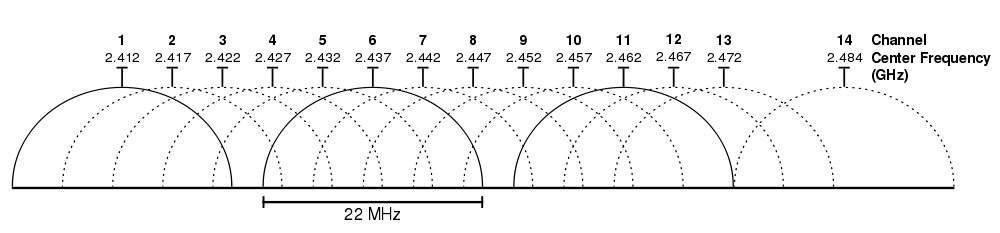
\includegraphics[width=0.8\textwidth]{figure/2GHz_WiFi_channels.png}
\caption{There are three channels that do not overlap in the on 2.4 GHz : 1, 6 and 11.} 
\label{fig:channels}
\end{figure}

In the 2.4 GHz band, 1, 6 and 11 are the only non-overlapping channels. Selecting one or more of these channels is an important part of setting up your network correctly. As we can see from Figure \ref{fig:channels}, co-channel interference is where devices take turns talking, so the more devices on one channel, the longer it takes for a device to talk since it has to wait for its turn. In our dataset we find that access points in this building mostly use channel 1, 6, and 11. Specifically, 42\% of access points use channel 6, 21\% of access points use channel 1, 28\% of access points use channel 11 and the rest use other overlapping channels. In general, we expect there are equal network traffic in channel 1, 6, 11, respectively. However,  many wireless routers automatically select the channel for you upon initial setup, it could lead to slow Wi-Fi speeds and interference. 